%%%%%%%%%%%%%%%%%%%%%%%%%%%%%%%%%%%%%%%%%
% University Assignment Title Page 
% LaTeX Template
% Version 1.0 (27/12/12)
%
% This template has been downloaded from:
% http://www.LaTeXTemplates.com
%
% Original author:
% WikiBooks (http://en.wikibooks.org/wiki/LaTeX/Title_Creation)
%
% License:
% CC BY-NC-SA 3.0 (http://creativecommons.org/licenses/by-nc-sa/3.0/)
%
%%%%%%%%%%%%%%%%%%%%%%%%%%%%%%%%%%%%%%%%%
%\title{Title page with logo}
%----------------------------------------------------------------------------------------
%	PACKAGES AND OTHER DOCUMENT CONFIGURATIONS
%----------------------------------------------------------------------------------------

\documentclass[12pt]{article}
\usepackage[english]{babel}
\usepackage[utf8x]{inputenc}
\usepackage{natbib}
\usepackage{color}
\usepackage[explicit]{titlesec}
\usepackage{url}
\usepackage{graphicx}
\usepackage[section]{placeins}


\begin{document}

\begin{titlepage}

\newcommand{\HRule}{\rule{\linewidth}{0.5mm}} % Defines a new command for the horizontal lines, change thickness here

\center % Center everything on the page
 
%----------------------------------------------------------------------------------------
%	HEADING SECTIONS
%----------------------------------------------------------------------------------------

\textsc{\LARGE University of St Andrews}\\[1.5cm] % Name of your university/college
\textsc{\Large CS5014 }\\[0.5cm] % Major heading such as course name
\textsc{\large Practical 1}\\[0.5cm] % Minor heading such as course title

%----------------------------------------------------------------------------------------
%	TITLE SECTION
%----------------------------------------------------------------------------------------

\HRule \\[0.4cm]
{ \huge \bfseries Machine Learning}\\[0.4cm] % Title of your document
\HRule \\[1.5cm]
 
%----------------------------------------------------------------------------------------
%	AUTHOR SECTION
%----------------------------------------------------------------------------------------


\Large \emph{Author:}\\
 \textsc{150008022}\\[3cm] % Your name

%----------------------------------------------------------------------------------------
%	DATE SECTION
%----------------------------------------------------------------------------------------

{\large \today}\\[2cm] % Date, change the \today to a set date if you want to be precise

%----------------------------------------------------------------------------------------
%	LOGO SECTION
%---------------------------------------------------------------------------------------


\includegraphics[width = 3.1cm]{images/standrewslogo.png}
 
%----------------------------------------------------------------------------------------

\vfill % Fill the rest of the page with whitespace

\end{titlepage}

\pagenumbering{gobble}

\part*{Goal}

The goal of this practical was to cleanse and process real world data in order to produce a regression model, and evaluate its performance.

\tableofcontents

\pagebreak

\pagenumbering{arabic}
\setcounter{page}{1}

\part{Loading and Cleaning the Data}

Numpy was used to load the csv file. The header row was skipped, and to ensure there were no missing values, the invalid raise flag was also used when parsing the data. This would raise an exception if any rows were found to be missing data. 

No preproccessing had occurred on the data set according to the original paper, and so the data could be used as given.

The input and output columns were separated into two variables x and y, in accordance with the notation used in lectures.

\part{Analysing and Visualising the Data}

Firstly, a histogram of each of the input variables and outputs were plotted in order to visualise the distribution of the values (Figures \ref{fig:xdist} and \ref{fig:ydist}). When comparing to the histograms from the given paper \cite{tsanas_xifara_2012}, most of the plots matched. Any differences were identified to be caused by 10 bins always being used (the default if not specified by numpy.hist), and the paper would sometimes use more. However, it was still clear that none of the variables had a gaussian distribution. The output variables also appeared tail heavy, but the inputs did not.

\begin{figure}[!ht]
\centering
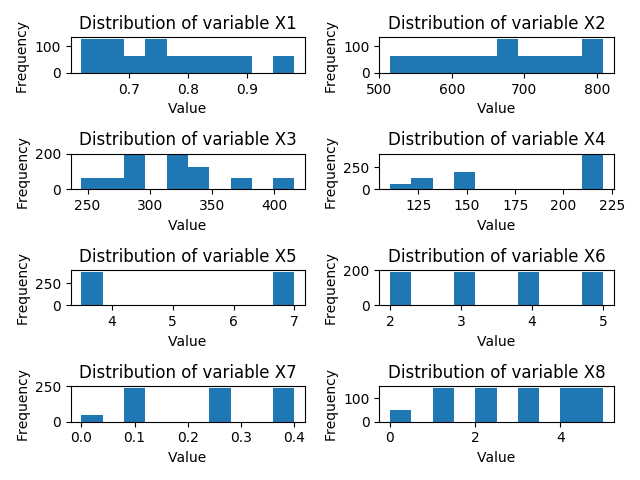
\includegraphics[width=0.8 \linewidth]{images/XDist}
\caption{Distribution of input variables}
\label{fig:xdist}
\end{figure}

\begin{figure}[!ht]
\centering
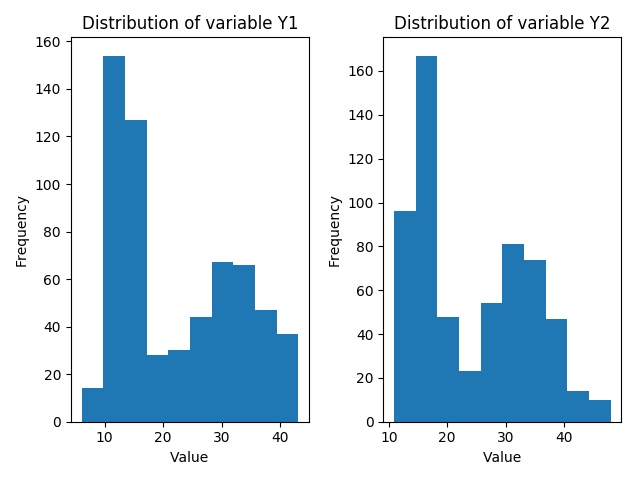
\includegraphics[width=0.8 \linewidth]{images/YDist}
\caption{Distribution of output variables}
\label{fig:ydist}
\end{figure}

\FloatBarrier

In order to identify which variables had the strongest relationships with the outputs, and if these relationships were linear or monotonic, scatter graphs were made between each input and output variable (Figures \ref{fig:xvsy0} and \ref{fig:xvsy1}). Feature scaling (specifically mean normalisation) was used to allow for comparisons between values that could have very different ranges. The resulting plots resembled those from the given paper, with different x-axis values since mean normalisation gave values in the range $-0.5 \leq x \leq 0.5 $. To better visualise the density of the data points as well as their position, the \url{alpha} parameter was set to 0.1 in the plots. 

\begin{figure}[!ht]
\centering
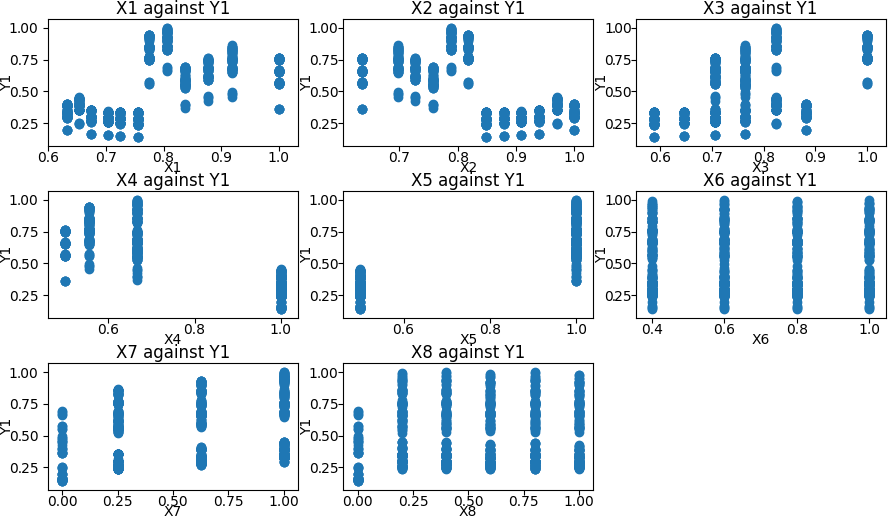
\includegraphics[width=0.8 \linewidth]{images/XsVsY0}
\caption{Normalised inputs plotted against the first output variable}
\label{fig:xvsy0}
\end{figure}

\begin{figure}[!ht]
\centering
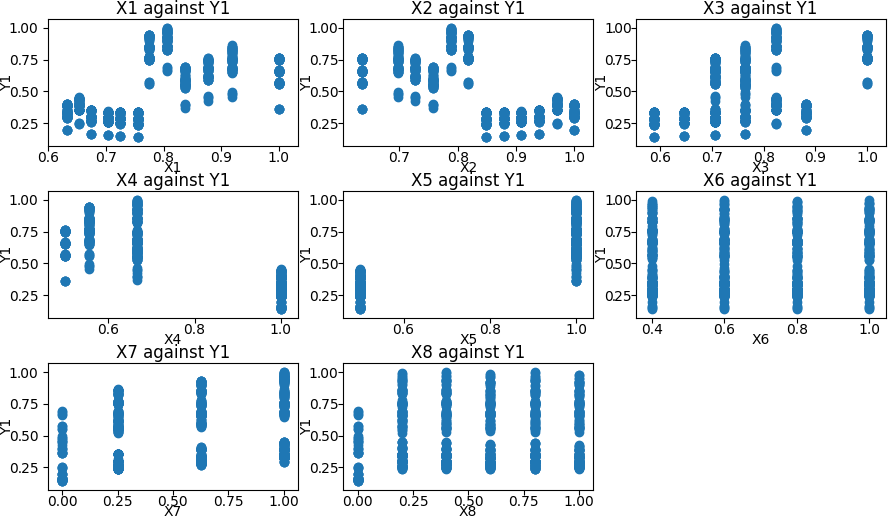
\includegraphics[width=0.8 \linewidth]{images/XsVsY0}
\caption{Normalised inputs plotted against the second output variable}
\label{fig:xvsy1}
\end{figure}

\FloatBarrier

Since the distribution of the outputs were so similiar, they were also plotted against each other in a scatter plot (Figure \ref{fig:y1vsy2}). This showed that the two variables had very similiar values, and so a regression model that applied to only one of them could likely be used for the other.

\begin{figure}[!ht]
\centering
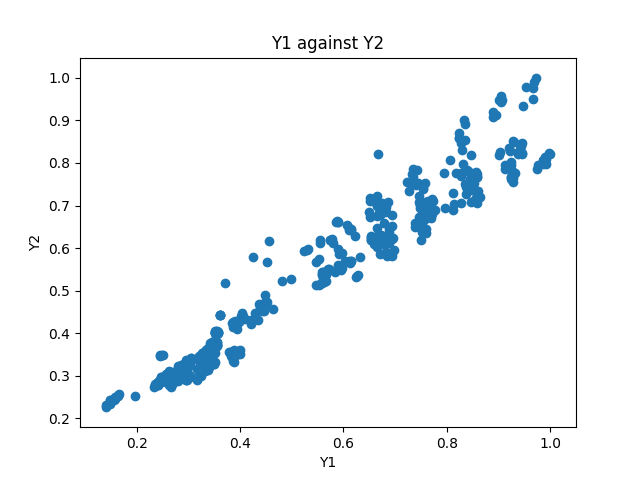
\includegraphics[width=0.8 \linewidth]{images/Y1vsY2}
\caption{Normalised outputs against each other}
\label{fig:y1vsy2}
\end{figure}

\FloatBarrier

\part{Feature Selection}

To try and identify which features had the strongest effect on the outputs, both the Pearson and Spearman rank correlation coefficients were considered. It was noted that the Pearson correlation would give a perfect value when the two variables were linearly related, whilst the Spearman correlation (a similiar alternative, and the one used in the original paper) would give a perfect value when the variables were monotonically related. Pearson is meant for use with continuous variables, whilst Spearman can be used for both continuous and ordinal variables, which our data set contains. Given these factors, the Spearman rank correlation coefficient was used as a filter method.

From the scatter plots, some variables appeared to have a possible linear relationship with the outputs (for example, X7 and Y1), whilst others had a monotonic relationship (for example, X1 and Y1). Using the Scipy \emph{stats.spearmanr} method, the correlation coefficients were easily calculated, alongside a p-value, as shown in table \ref{tbl:spearman-table}. Immediately from these result we can see that X6 and X8 show little evidence of a monotonic relationship existing between them and either of the outputs. This can also be seen from the scatter plots.

Given more time and better knowledge of the subject matter, it may be possible to merge correlated features instead of remove them in order to reduce the number of dimensions of our input. 

\begin{table}[!ht]
\centering
\caption{Spearman rank correlation coefficients, with p values}
\label{tbl:spearman-table}
\begin{tabular}{||llll||}
\hline
X    				& Y & Rho   & p    \\
\hline
1                   & 1 & 0.62  & 0.00 \\
1                   & 2 & 0.65  & 0.00 \\
2                   & 1 & -0.62 & 0.00 \\
2                   & 2 & -0.65 & 0.00 \\
3                   & 1 & 0.47  & 0.00 \\
3                   & 2 & 0.42  & 0.00 \\
4                   & 1 & -0.80 & 0.00 \\
4                   & 2 & -0.80 & 0.00 \\
5                   & 1 & 0.86  & 0.00 \\
5                   & 2 & 0.86  & 0.00 \\
6                   & 1 & -0.00 & 0.91 \\
6                   & 2 & 0.02  & 0.63 \\
7                   & 1 & 0.32  & 0.00 \\
7                   & 2 & 0.29  & 0.00 \\
8                   & 1 & 0.07  & 0.06 \\
8                   & 2 & 0.05  & 0.20 \\
\hline
\end{tabular}
\end{table}

Given the number of input features, using them all would have negative effects on the choosen algorithm. Including each feature could result in overfitting, and would require more training data to eliminate this issue. It would also increase the computation time required to train our model. Features that have no real effect on the outputs would also act simply as noise, which would negatively effect our model. And since the amount of available data is small, it would be preferable to use fewer features.

Recursive Feature Elimination was then also considered to help choose which features were important. It does this by creating models using subsets of the features, determining the worst performing feature from both subsets, removing it, and then repeating this process recursively until a specific number of features are left. Using the \emph{RFE} class from sklearn, this was done fairly simply, and when asked to identify the 4 best performing features for both Y1 and Y2, it eliminated X1 and X2. 

Next, the testing set was to be isolated from the available data. Simple random sampling (SRS) and stratified sampling were considered for performing our data splitting. SRS is intuitive, but for less uniformly distributed data sets, it can lead to subsets that poorly represent the input data, and therefore suffer from sampling bias \cite{reitermanova_2010}. 

For these reasons, stratified random sampling was used with a 80\%-20\% split. In order to do so, the data would have to first be split into seperate strata. To ensure our training and testing sets were representative of our data, the output variables were used to categorise the data into strata. Since the two appeared to have a linear relationship as shown in figure \ref{fig:y1vsy2}, we could assume that using one column for categorising our data would produce an equal distribution of the values in both columns.

The 586 possible values of Y1 were split into 50 bins using \url{numpy.digitize}, and then passed to \url{train_test_split} as the \url{stratify} argument. Scatter plots of the training data and test data were used to confirm that this method of stratifying did capture most features of the data. 

\part{Selecting and Training a Regression Model}

The limited size of the corpus available made the choice of algorithm especially crucial. The lack of noticable outliers in the visualistions at least suggest that the data is not of poor-quality. Due to the small corpus size, K-fold cross-validation was chosen to estimate the model error \cite{gron_2018}. 

Root Mean Square Error (RMSE) and Mean Absolute Error (MAE) were both considered as performance measures for regression. RMSE is more sensitive to outliers, but is generally preffered when absent, which is true for our input, and so it was chosen. 


\part{Performance Evaluation}

\part{Discussion}

\part{Conclusion}

\bibliographystyle{unsrt}
\bibliography{mybib}

\end{document}
